% ======================================================================
% 5. přednáška (31. 10. 2022) – Interakce záření s látkou, kosmické záření
% ======================================================================
\section{Interakce fotonů a nabitých částic s látkou}

\strana{P05-1}
Abychom mohli jakoukoli částici \emph{detekovat}, musí v detektoru zanechat
nějakou stopu – a stopu zanechá jen tehdy, když s látkou detektoru
interaguje. Stejné procesy navíc určují, jak se záření stíní a jak škodí
živé tkáni (k tomu se dostaneme v další přednášce). Proto se nyní podíváme
na to, jakými mechanismy ztrácejí energii fotony a nabité částice při
průchodu látkou. Davídkovy slajdy (kapitola „Interakce částic s látkou
a detektory`` ) odkazují pro podrobné vzorce a grafy na tabulky Particle
Data Group (\texttt{pdg.lbl.gov}).

\subsection{Interakce fotonů}

Foton nemá náboj, a proto neztrácí energii postupně (po malých kouscích
v mnoha srážkách) jako nabitá částice. Naopak: foton buď proletí beze
změny, nebo v jediné interakci zmizí (fotoefekt, tvorba párů) či se
výrazně odkloní (rozptyl). Pravděpodobnost, že foton „přežije`` tloušťku
\(x\), je proto stejná na každém dalším úseku dráhy a svazek je zeslabován
exponenciálně:
\[
  \vzorec{I(x) = I(0)\,e^{-x/\lambda} = I(0)\,e^{-x n\sigma}}
\]
Zde \(I(0)\) je intenzita dopadajícího svazku, \(I(x)\) intenzita svazku,
který prošel vrstvou tloušťky \(x\) bez interakce, \(n\) je počet terčových
center (atomů) v jednotce objemu a \(\sigma\) celkový účinný průřez pro
interakci fotonu s jedním atomem (součet přes všechny mechanismy níže).
Veličina
\(\lambda = 1/(n\sigma)\) je \kw{střední volná dráha} (absorpční délka)
– na vzdálenosti \(\lambda\) klesne intenzita na \(1/e\).

\begin{vysvetleni}[Odkud se bere exponenciála]
Na tenké vrstvě \(\dd x\) interaguje podíl \(n\sigma\,\dd x\) fotonů (terčové
plošky \(\sigma\) zakrývají z jednotkové plochy právě zlomek
\(n\,\dd x\,\sigma\)). Tedy \(\dd I = -I\,n\sigma\,\dd x\), a integrací
\(I(x) = I(0)\,e^{-n\sigma x}\). Je to stejná logika jako u radioaktivního
rozpadu: „bezpaměťový`` proces s konstantní pravděpodobností na jednotku
dráhy. V praxi se tloušťka často udává v g\,cm\(^{-2}\) (tj. \(\rho x\))
a místo \(n\sigma\) se používá hmotnostní součinitel zeslabení
\(\mu/\rho\); viz shrnutí cvičení.
\end{vysvetleni}

Hlavní \kw{mechanismy} interakce fotonů s látkou jsou:
\begin{itemize}
  \item fotoefekt,
  \item Comptonův rozptyl,
  \item Rayleighův rozptyl,
  \item tvorba párů \(e^+e^-\).
\end{itemize}
Který z nich převládá, záleží hlavně na energii fotonu \(E_\gamma\)
a na protonovém čísle \(Z\) látky: zhruba fotoefekt dominuje do stovek keV,
Comptonův rozptyl v oblasti \(\sim\)\,MeV a tvorba párů nad několika MeV
(pro olovo jsou hranice níže, pro lehké látky výše).

\subsubsection{Fotoefekt}
\[
  \gamma + X \;\to\; X^{+} + e^-
\]
Foton je atomem \(X\) celý pohlcen a jeho energie se předá jednomu
z vázaných elektronů, který je vyražen (nejčastěji z K-slupky; ionizovaný
atom pak deexcituje vyzářením charakteristického rentgenového záření,
viz Davídkovy slajdy „Interakce fotonů``). Kinetická energie elektronu je
\(E_\gamma - E_{\text{vazby}}\). Proces nemůže proběhnout na volném
elektronu – nešlo by současně zachovat energii a hybnost – potřebujeme
atom (jádro), které převezme zpětný ráz. Proto fotoefekt silně závisí na
tom, jak pevně (a jak blízko jádra) jsou elektrony vázány.
\begin{itemize}
  \item \kw{Rezonanční charakter}: účinný průřez má ostré skoky
  (absorpční hrany K, L, \dots) – jakmile energie fotonu překročí vazebnou
  energii další slupky, otevře se nový kanál a \(\sigma\) skokem vzroste.
  \item Mezi hranami účinný průřez strmě klesá s energií a velmi silně roste
  se \(Z\):
  \[
    \vzorec{\sigma_{\text{f}} \sim Z^5\,E_\gamma^{-7/2}}
  \]
\end{itemize}
Silná závislost \(\sim Z^5\) je důvod, proč se ke stínění nízkoenergetického
\(\gamma\) a rentgenového záření používá olovo a proč jsou na rentgenovém
snímku vidět kosti (vápník má vyšší \(Z\) než měkká tkáň).

\subsubsection{Rayleighův rozptyl}
\[
  \sigma \sim \lambda^{-4}
\]
(\(\lambda\) je zde vlnová délka fotonu.) Jde o \pozor{pružný} rozptyl
nízkoenergetických fotonů: foton „rozkmitá`` elektronový obal celého atomu,
který pak vyzáří foton \emph{stejné} energie, jen v jiném směru.
\begin{itemize}
  \item \oprava{koherentní}{nekoherentní} rozptyl na celém atomu, významný
  pro \(E_\gamma < 10\,\text{keV}\).
\end{itemize}
Závislost \(\lambda^{-4}\) je stejná jako v klasické optice (proto je obloha
modrá). Protože se energie fotonu nemění a atom není ionizován, Rayleighův
rozptyl nezanechává v látce stopu – pouze mění směr svazku.

\begin{vysvetleni}[Proč „koherentní``]
Rayleighův rozptyl se v literatuře (i v tabulkách PDG/NIST XCOM) nazývá
\emph{koherentní} rozptyl: všechny elektrony atomu přispívají ve fázi
a atom zůstává ve stejném stavu (Davídkovy slajdy: „Rayleighův (pružný)
rozptyl``). \emph{Nekoherentní} rozptyl je naopak název pro Comptonův
rozptyl na jednotlivých elektronech. V poznámkách jsou tedy pojmy zřejmě
prohozeny.
\end{vysvetleni}

\subsubsection{Comptonův rozptyl}
Foton se rozptýlí na \emph{kvazivolném} elektronu (vazebná energie vnějších
elektronů je zanedbatelná vůči \(E_\gamma\)), předá mu část své energie
a odletí pod úhlem \(\theta\):

\begin{center}
\begin{tikzpicture}[>=Stealth, thick]
  \draw[decorate,decoration={snake,amplitude=2.5pt,segment length=8pt}] (0,0) -- (2.3,0);
  \draw[->] (2.3,0) -- (2.45,0);
  \fill (2.5,0) circle (2.5pt) node[below left] {\(e^-\)};
  \draw[dashed, thin] (2.5,0) -- (4.5,0);
  \draw[decorate,decoration={snake,amplitude=2.5pt,segment length=8pt}] (2.5,0) -- (4.1,1.1);
  \draw[->] (4.1,1.1) -- (4.25,1.2) node[right] {\(\gamma'\)};
  \draw[->] (2.5,0) -- (3.8,-1.3) node[below right] {\(e^-\)};
  \draw[->, thin] (3.4,0) arc (0:34:0.9);
  \node at (3.65,0.3) {\(\theta\)};
  \node at (0.5,0.35) {\(\gamma\)};
\end{tikzpicture}
\end{center}

Ze zákonů zachování čtyřhybnosti (v jednotkách \(c=1\)) plyne energie
rozptýleného fotonu
\[
  \vzorec{E'_\gamma = \frac{E_\gamma}{1 + \dfrac{E_\gamma}{m_e}\,(1-\cos\theta)}}
\]
kde \(m_e\) je hmotnost elektronu (\(511\,\text{keV}\)). Pro
\(E_\gamma \ll m_e\) je \(E'_\gamma \approx E_\gamma\) (limita klasického
Thomsonova rozptylu), pro \(E_\gamma \gg m_e\) ztrácí foton při rozptylu
dozadu (\(\theta=\pi\)) téměř všechnu energii,
\(E'_\gamma \to m_e/2\). Maximální energie předaná elektronu určuje tzv.
Comptonovu hranu ve spektru detektoru.

\begin{vysvetleni}[Odvození Comptonova vzorce]
Označme čtyřhybnosti \(k, k'\) (foton před/po), \(p=(m_e,\vec 0)\) a \(p'\)
(elektron). Ze zachování \(p' = p + k - k'\) a \(p'^2 = m_e^2\) dostaneme
\(m_e^2 = m_e^2 + 2p\cdot k - 2p\cdot k' - 2k\cdot k'\) (neboť \(k^2=k'^2=0\)).
Tedy \(m_e E_\gamma - m_e E'_\gamma = E_\gamma E'_\gamma(1-\cos\theta)\),
odkud plyne vzorec výše. V obvyklých jednotkách:
\(\lambda' - \lambda = \frac{h}{m_e c}(1-\cos\theta)\).
\end{vysvetleni}

\begin{itemize}
  \item Účinný průřez na atom:
  \[
    \sigma_{\text{C}} \sim Z/E
  \]
  Faktor \(Z\) vyjadřuje prostě počet elektronů v atomu (rozptyl probíhá na
  každém zvlášť), pokles \(1/E\) (přesněji \(\sim \ln E/E\) pro velká \(E\))
  plyne z Klein–Nishinova vzorce.
\end{itemize}

\strana{P05-2}
\subsubsection{Tvorba párů}
Foton s dostatečnou energií se v poli jiné nabité částice přemění na pár
elektron–pozitron. Ve vakuu to nejde: volný foton nemůže současně zachovat
energii i hybnost při přeměně na masivní pár, potřebuje „partnera``, který
převezme hybnost.

\begin{center}
\begin{tikzpicture}[>=Stealth, thick]
  % v poli jadra
  \draw[decorate,decoration={snake,amplitude=2.5pt,segment length=8pt}] (0,0) -- (1.9,0);
  \draw[->] (1.9,0) -- (2.05,0);
  \node at (0.9,-0.4) {\(\gamma\)};
  \fill (2.2,0) circle (2.5pt) node[below=2pt] {\(A\)};
  \draw[->] (2.35,0.05) -- (3.6,0.8) node[right] {\(e^+\)};
  \draw[->] (2.35,-0.05) -- (3.6,-0.6) node[right] {\(e^-\)};
  % v poli elektronu
  \fill (2.2,-2) circle (2.5pt) node[below=2pt] {\(e^-\)};
  \draw[->] (2.35,-1.95) -- (3.6,-1.5) node[right] {\(e^-\)};
  \draw[->] (2.35,-2.05) -- (3.6,-2.8) node[right] {\(e^+\)};
  % popisky
  \node[right, align=left] at (5,0.1) {\(\sigma \sim Z^2 \ln E_\gamma\), \quad \(E_\gamma > 2m_e\)};
  \node[right, align=left] at (5,-2.1) {\(\sigma \sim Z \ln E_\gamma\), \quad \(E_\gamma > 4m_e\)};
\end{tikzpicture}
\end{center}

\begin{itemize}
  \item \emph{V poli jádra} \(A\) (pravděpodobnější):
  \[
    \vzorec{\sigma \sim Z^2 \ln E_\gamma, \qquad E_\gamma > 2m_e}
  \]
  Jádro je těžké, takže převezme hybnost téměř bez energie – práh je dán
  jen klidovou energií páru, \(2m_e = 1{,}022\,\text{MeV}\). Faktor \(Z^2\)
  pochází z toho, že amplituda je úměrná náboji jádra \(Ze\) (Coulombovo
  pole), účinný průřez jejímu kvadrátu.
  \item \emph{V poli elektronu} (atomového):
  \[
    \sigma \sim Z \ln E_\gamma, \qquad E_\gamma > 4m_e
  \]
  Elektronů je v atomu \(Z\), každý má jednotkový náboj, proto jen \(\sim Z\).
  Práh je vyšší, protože lehký elektron při zpětném rázu odnese podstatnou
  energii – v koncovém stavu jsou tři částice o hmotnosti \(m_e\).
\end{itemize}

\begin{vysvetleni}[Proč práh \(4m_e\)]
Práh se spočte z invariantní hmoty: počáteční stav \(\gamma + e^-\) (elektron
v klidu) má \(s = m_e^2 + 2m_eE_\gamma\); koncový stav \(e^-e^+e^-\) má
minimálně \(\sqrt s = 3m_e\). Z \(m_e^2 + 2m_eE_\gamma = 9m_e^2\) plyne
\(E_\gamma = 4m_e\). Pro jádro o hmotnosti \(M\) analogicky
\(E_\gamma = 2m_e(1 + m_e/M) \approx 2m_e\).
\end{vysvetleni}

Při vysokých energiích je tvorba párů dominantním procesem; spolu
s brzdným zářením vytváří elektromagnetické spršky a charakterizuje se
radiační délkou \(X_0\) (s ní budeme počítat v příští přednášce).

\subsection{Interakce nabitých částic}

Nabitá částice na rozdíl od fotonu interaguje coulombovsky neustále
– s každým elektronem, kolem něhož proletí – a ztrácí tedy energii
spojitě, po malých kouscích. Mechanismy:
\begin{itemize}
  \item \kw{excitace} – vybuzení elektronu atomu na vyšší hladinu, při
  deexcitaci se vyzáří foton;
  \item \kw{ionizace} – uvolnění elektronu, vznikají volné elektrony
  a kladné ionty (tyto náboje pak sbírají ionizační detektory);
  \item \kw{brzdné záření} – vyzáření fotonu při urychlení částice
  v Coulombově poli jádra (významné hlavně pro lehké elektrony);
\end{itemize}
\vspace{-4pt}\noindent\rule{3cm}{0.4pt}

První tři procesy jsou z hlediska energetických ztrát hlavní (ionizační
ztráty těžkých částic popisuje Bethe–Blochova formule, viz Davídkovy slajdy
„Interakce nabitých částic (2)``). Následující tři naopak k ztrátám
energie přispívají málo, ale jsou \pozor{zajímavé pro detekci}:
\begin{itemize}
  \item \kw{Čerenkovovo záření},
  \item \kw{přechodové záření} – vzniká při průchodu částice rozhraním dvou
  prostředí s různým indexem lomu,
  \item \kw{scintilace} – část energie excitace molekul/krystalu se vyzáří
  ve viditelné oblasti; světlo pak zaznamenáme fotonásobičem.
\end{itemize}

\subsubsection{Čerenkovovo záření}
Letí-li nabitá částice prostředím rychleji, než je fázová rychlost světla
v tomto prostředí (\(v > c/n\), tj. \(\beta > 1/n\), kde \(n\) je index lomu),
vyzařuje kužel světla – optickou obdobu nadzvukového „třesku``. Světlo
vychází pod pevným úhlem \(\theta_c\) vzhledem ke směru letu:

\begin{center}
\begin{tikzpicture}[>=Stealth, thick]
  \draw[->] (0,0) -- (5,0) node[below] {\(e^-\)};
  \foreach \s in {0.8,1.6} {
    \draw[decorate,decoration={snake,amplitude=2pt,segment length=7pt}] (\s,0) -- ++(35:2.6);
    \draw[->] ($(\s,0)+(35:2.6)$) -- ++(35:0.2);
    \draw[decorate,decoration={snake,amplitude=2pt,segment length=7pt}] (\s,0) -- ++(-35:2.6);
    \draw[->] ($(\s,0)+(-35:2.6)$) -- ++(-35:0.2);
  }
  \draw[thin] (2.7,0) arc (0:35:1.1);
  \node at (3.0,0.33) {\(\theta_c\)};
\end{tikzpicture}
\end{center}

\[
  \vzorec{\cos\theta_c = \frac{1}{\beta n}}, \qquad I(\theta_c) \sim \sin^2\theta_c .
\]
Geometricky: za čas \(t\) urazí částice dráhu \(\beta c t\), zatímco vlna
vyzářená na začátku doletí do vzdálenosti \(ct/n\); obálka vln tvoří kužel
s \(\cos\theta_c = (ct/n)/(\beta ct)\). Intenzita (počet vyzářených fotonů na
jednotku dráhy, Frankův–Tammův vzorec) je úměrná \(\sin^2\theta_c\): těsně nad
prahem (\(\beta n \to 1\), \(\theta_c\to 0\)) částice nezáří téměř vůbec.
Energetické ztráty Čerenkovovým zářením jsou zanedbatelné (\(<1\,\%\)
ionizačních), ale úhel \(\theta_c\) přímo měří rychlost \(\beta\) – a to je
pro detekci velmi cenné.

\begin{priklad}[Rozlišení \(p\) a \(\pi\) o hybnosti \(10\,\text{GeV}\) – prahový Čerenkovův detektor]
Proton a pion se stejnou hybností \(p = 10\,\text{GeV}\) mají různé rychlosti,
protože mají různé hmotnosti (\(\beta = p/E = p/\sqrt{p^2+m^2}\)):
\[
  \beta_p = \frac{10}{\sqrt{100 + 0{,}938^2}} \approx 0{,}9956, \qquad
  \beta_\pi = \frac{10}{\sqrt{100 + 0{,}140^2}} \approx 0{,}99990 .
\]
Zvolíme-li radiátor (typicky plyn, jehož index lomu lze měnit tlakem) tak,
aby práh \(1/n\) ležel \emph{mezi} oběma rychlostmi, tj.
\(1{,}0001 \lesssim n \lesssim 1{,}0044\), bude zářit jen pion; proton
(zakroužkován) zůstane pod prahem.

\begin{center}
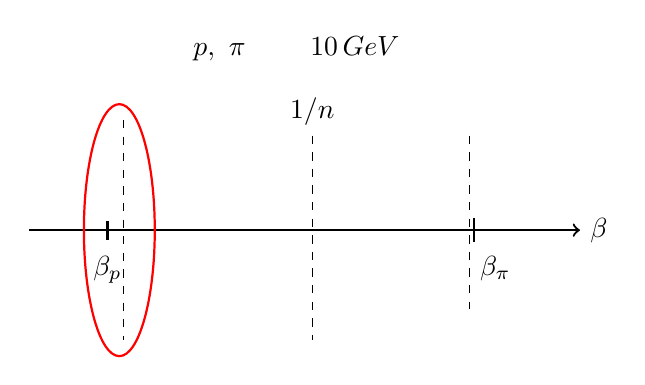
\begin{tikzpicture}[thick]
  \draw[->] (0,0) -- (7,0) node[right] {\(\beta\)};
  \draw (1,0.12) -- (1,-0.12);
  \draw[dashed, thin] (1.2,1.4) -- (1.2,-1.4);
  \node[below] at (1.0,-0.2) {\(\beta_p\)};
  \draw[red, thick] (1.15,0) ellipse (0.45 and 1.6);
  \draw[dashed, thin] (3.6,1.2) -- (3.6,-1.4);
  \node[above] at (3.6,1.2) {\(1/n\)};
  \draw[dashed, thin] (5.6,1.2) -- (5.6,-1.0);
  \draw (5.65,0.15) -- (5.65,-0.15);
  \node[below right] at (5.6,-0.2) {\(\beta_\pi\)};
  \node at (3.4,2.3) {\(p,\ \pi\) \qquad \(10\,\text{GeV}\)};
\end{tikzpicture}
\end{center}
\pozn{Prostřední čárkovanou čáru v náčrtku interpretuji jako práh \(1/n\);
v originále není popsána.}
\end{priklad}

\subsection{Kosmické záření}

Primární kosmické záření jsou převážně vysokoenergetické protony. Vysoko
v atmosféře interagují s jádry vzduchu a vytvářejí spršky; na povrch Země
dopadají hlavně miony \(\mu^\pm\) z rozpadů nabitých pionů (Davídkovy slajdy
„Kosmické záření (2)``: střední energie \(\langle E_\mu\rangle \approx 4\,\text{GeV}\),
tok \(\approx 70\,\text{m}^{-2}\text{s}^{-1}\text{sr}^{-1}\)). Ukážeme si dva
jednoduché odhady: kolik energie mion v atmosféře ztratí a (v příští přednášce)
jaká část mionů se cestou nerozpadne.

\begin{priklad}[Kolik energie ztratí mion v atmosféře?]
Mion je těžká nabitá částice, která v atmosféře ztrácí energii téměř jen
ionizací. Pro relativistické částice (\(\beta\gamma \sim 3\)–\(100\)) jsou
ionizační ztráty blízko minima Bethe–Blochovy křivky a vyjádřené na
jednotku plošné hustoty jsou téměř nezávislé na materiálu:
\[
  \frac{\Delta E}{\Delta x\,\rho} \sim 2\,\text{MeV}\cdot\text{g}^{-1}\text{cm}^2 .
\]
Atmosféra představuje stejné množství hmoty na \(\text{cm}^2\) jako
\(10\,\text{m}\) vodního sloupce (výška vodního sloupce odpovídající
atmosférickému tlaku, \(p = \rho g h \approx 10^5\,\text{Pa}\)). Tedy
\[
  \Delta E(\mu) = 2\,\frac{\text{MeV}}{\text{g}\cdot\text{cm}^{-2}}
  \cdot \underbrace{1\,\text{g}\cdot\text{cm}^{-3}}_{\mathrm{H_2O}}
  \cdot 10\,\text{m} = 2\,\text{GeV}.
\]
(\(10\,\text{m} = 1000\,\text{cm}\), takže
\(2\,\text{MeV}\cdot 1000 = 2\,\text{GeV}\).) Mion, který má dorazit na zem
s typickou energií \(\sim 4\,\text{GeV}\), musel tedy vzniknout s energií
\(\sim 6\,\text{GeV}\) – s touto hodnotou počítáme v příští přednášce.
\end{priklad}
